%%%%%%%% ICML 2021 EXAMPLE LATEX SUBMISSION FILE %%%%%%%%%%%%%%%%%
\documentclass{article}
\usepackage[]{algorithm2e}
\usepackage{algorithmic}
\usepackage{algorithm}
% Recommended, but optional, packages for hs and better typesetting:
\usepackage{microtype}
\usepackage{graphicx}
\usepackage{amsmath}
\usepackage{appendix}
\usepackage{subfigure}
\usepackage{booktabs} % for professional tables
\usepackage{hyperref}
% Attempt to make hyperref and algorithmic work together better:
\newcommand{\theHalgorithm}{\arabic{algorithm}}
\usepackage{icml2021}
\usepackage{float}
\usepackage{enumitem}

\begin{document}
\twocolumn[
\icmltitle{Reinforcement Learning 2024
Assignment 3: Policy-based Reinforcement Learning}

\icmlsetsymbol{equal}{*}
\begin{icmlauthorlist}
\icmlauthor{Sherry Usman}{equal,to}
\icmlauthor{Qin Zhipei}{equal,to}
\icmlauthor{Megan Mirnalini Sundaram R}{equal, to}
\end{icmlauthorlist}

\icmlaffiliation{to}{Leiden University}

% You may provide any keywords that you
% find helpful for describing your paper; these are used to populate
% the "keywords" metadata in the PDF but will not be shown in the document
\icmlkeywords{Machine Learning, Deep Q-Learning, Experience Replay, Target Network}

\vskip 0.3in
]

\begin{abstract}

\end{abstract}

\section {Introduction}
In this paper we will delve into the Lunar Lander environment taken from the OpenAI Gym library. The Lunar Lander game is a classical reinforcement learning environment where the goal is to optimise the trajectory of a rocket such that it lands between the two flags. 

\begin{figure}[htbp]
\centering
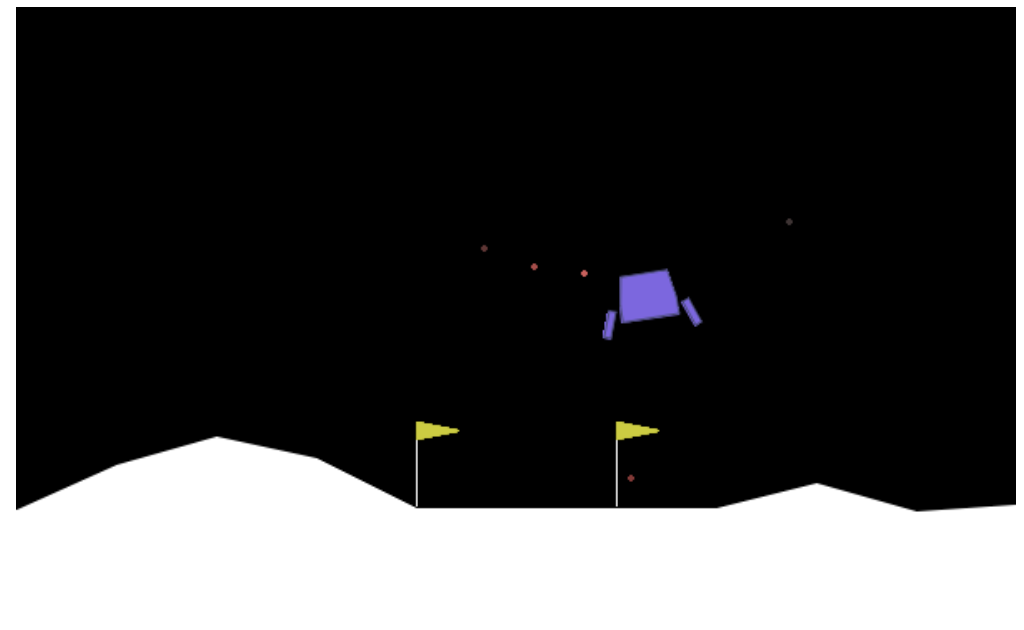
\includegraphics[width=0.6\linewidth]{Report/images/visualisation.png}
\caption{\label{fig:Visualization of the Cart-pole} A visualisation of the Lunar Lander problem}
\end{figure}



The action space of the lunar lander environment is shown below. 
As seen below there are 4 potential actions: 0,1,2 and 3. 

\begin{table}[htbp]
\centering
\begin{tabular}{|l|c|}
\hline
\textbf{Value} & \textbf{Action} \\
\hline
0  & Do nothing \\
\hline
1 & fire left orientation engine \\
\hline
2  & fire main engine \\
\hline
3 & fire right orientation engine  \\
\hline
\end{tabular}
\caption{Action Space}
\label{tab:hyper-parameters}
\end{table}

The observation space is an 8-dimensional vector, the positional coordinates of the lunar lander (x and y), its linear velocities in x and in y respectively, its angle, its angular velocities and two boolean values that represent whether each leg is in contact with the ground or not. 

\section{Policy-Based Reinforcement Learning}
The policies we looked at in the previous papers were \emph{value-based}. This means that they looked at state-value pairs in the environment and approximated the rewards of such pairs using different exploration strategies like Boltzmann or Epsilon-Greedy. Policy based reinforcement learning are another genre of reinforcement learning algorithms. Used primarily in  continuous action space RL environments, policy-based reinforcement learning do not utilise a value function to determine the next best possible action. Instead, they use a parameterized policy. A value function may be used for learning the best policy, but not for selecting the action. The implemented policy is then improved, based on the data from each episode using policy gradient methods \cite{sutton-barlo}.
The outline of policy-based algorithms is using a parameterized policy function, which is denoted by $\pi_\Theta$. 
Here, $\theta$ refers to the parameters of the function and $\pi$ refers to the function itself. After defining the policy function, a path $\tau$ is chosen. If $\tau$ is good, then the parameters $\theta$ are increased towards the path $\tau$. Otherwise, it is decreased. In this way, it is maintained until the goal is reached.    \cite{plaat-deeprl}
The various algorithms that were implemented to realise this approach are:
\begin{itemize}
\item REINFORCE
\item Actor-Critic
\item Actor-Critic with baseline subtraction
\item Actor-Critic with bootstrapping
\item Actor Critic with bootstrapping and baseline subtraction
\end{itemize}
These algorithms are discussed in detail below. 

\subsection{REINFORCE}
\quad REINFORCE is a commonly used classic Monte-Carlo Policy Gradient algorithm. It is termed Monte-Carlo because it learns from the collected episodes by estimating gradients throughout the agent trajectory. We can recall the policy function  $\pi_{\theta}(a,s)$ which indicates the probability of taking an action a in the state s with the parameters $\theta$.
The REINFORCE algorithm optimises the policy function $\pi_{\theta}(a,s)$ by fine-tuning its parameters $\theta$ such that it increases the likelihood of actions with higher rewards. It does this by calculating the total expected rewards with respect to a particular parameter value $\theta$ and adjusting $\theta$ accordingly. Thus the parameters are updated as follows: \newline
\begin{equation}
\theta = \theta + \alpha\nabla\theta J(\theta). % ad the triangel her e
\end{equation}

where $\alpha$ is the learning rate, J($\theta$) is the expected return function which gives the total expected reward over all trajectories. 

As mentioned above, the parameters of the policy is defined by $\theta$. Therefore, the quality of such parameters for the state to action probabilities for the policy is given by $J(\theta)$. To improve the gradient, the differential of the parameters are taken. 

\newline The quality is given by $\mathbb{E}_\pi [ \sum _a q_\pi(S_t, a)\nabla_\pi(a|S_t, \theta)]$

\newline The update of these functions happen in a Monte-Carlo function i.e., random sample. The function is updated after an entire trajectory/path is completed. Therefore, this happens in an off-policy way.  

\subsection{Actor-Critic Methods}
 Actor Critic methods are TD methods and have a separate memory structure to store the policy independent of the value function. Thus it has two  structures/neural networks: a policy structure known as an \emph{actor} and an estimated value function known as the \emph{critic}. While the actor follows the policy and takes actions according to the policy, the critic, typical of its name, criticises the actions taken by the actor in the form of a TD error. This scalar signal indicates whether the actions taken by the agent are better or worse than what the critic expected. The TD error can be evaluated as follows in the following equation: \newline
 $\delta_{t} = R_{t+1} + \gamma * V_t(S_{t+1})-V_t(S_t)$ \newline
 where $\delta_{t}$ is the temporal difference error at timestep $t$, $R_{t+1}$ is the reward for transitioning from state $S_t$ to the state $S_{t+1}$,  $\gamma$ is the discount factor, $V_{t}$ is the value function from the critic and $V_t(S_{t+1})$ is the estimated value of going to state $S_{t+1}$ while $V_t(S_t)$ is the estimated value of going to state $S_t$.  \newline 
 Thus, a positive TD error indicates that the transition from state $S_t$ to $S_{t+1}$ is fruitful/ has a postive reward while a negative TD error indicates that the transition from state  $S_t$ to $S_{t+1}$ to $S_{t+1}$ is not rewarding.
 \newline


Unlike REINFORCE, Actor-critic Methods consists of two functions - the actor and the critic. The actor refers to the policy function and the critic refers to the value functions. Similar to an actor and a critic, the actor (policy) function focuses on the path to be taken, and the critic evaluates the said path, by computing the value function. 
The focus on the algorithms is based on policy gradients. \cite{actor-critic}
\newline As used in REINFORCE, the policy gradient is given by 
\newline 
$\nabla_\theta J(\theta) = \mathbb{E}_\pi[\sum _{t=0}^{T-1} \nabla_\theta log\pi_\theta (a_t|s_t)G_t]$
\subsubsection{Bootstrapping}
Actor Critic with bootstrapping is a particular actor-critic algorithm that combines the benefits of both value based (using state-action pairs) and policy based methods. Thus the inclusion of elements from value-based reinforcement learning bootstraps or supports the policy-based traditional Actor-critic method by counteracting the low bias and high variance. It combines the advantage of having a low variance from the value method, and the advantage of having a high bias from the policy method.
Similar to the traditional actor critic method, there is an actor who learns the policy and there is a critic which criticises/evaluates the rewards gained from following the policy (the value of particular state-action pairs Q(s,a)) . However, in the case of Actor Critic with bootstrapping, the critic uses bootstrapping to update the value Q of the state-action pairs, harking back to value-based methods. \newline 
particular state-action pairs  the actions taken by teh agent oin the form of a TD error. However, the critic 
However, there might be high variance in the rewards and gradient estimate. To counteract this, bootstrapping is used. 

\subsubsection{Baseline Subtraction}
Actor-Critic algorithms could also employ baseline subtraction which is a technique used to reduce the variance by using a baseline. We recall the previous policy gradient function denoted by $\nabla_\theta J(\theta) = \mathbb{E}_\pi[\sum _{t=0}^{T-1} \nabla_\theta log\pi_\theta (a_t|s_t)G_t]$. By subtracting a baseline $b(s_t)$ from the cumulative reward helps reduce make them smaller and more stable, reducing variance. The updated policy gradient function after baseline subtraction is shown below. 

$\nabla_\theta J(\theta) = \mathbb{E}_\pi[\sum _{t=0}^{T-1} \nabla_\theta log\pi_\theta (a_t|s_t)G_t - b(s_t)]$



\subsubsection{Bootstrapping and Baseline Subtraction}


\section{Goals Achieved}
\subsection{Effects of policy gradients on variance}
\subsection{Effects of bootstrapping on the policy gradients}
\subsection{Comparison of Performance}
\subsection{Effect of entropy regularization on performance}

\bibliography{Report/references}
\bibliographystyle{Report/reference_style}
\end{document}

